
\section*{CHƯƠNG 2. HƯỚNG DẪN SỬ DỤNG}
\setcounter{section}{2}
\setcounter{subsection}{0} %LƯU Ý MỖI LẦN THÊM CHƯƠNG MỚI CẦN THÊM CÂU NÀY ĐỂ RESET THỨ TỰ CỦA SUBSECTON VỀ 1
\setcounter{table}{0} % LƯU Ý SAU MỖI LẦN GỌI BẢNG HAY HÌNH ẢNH PHẢI THÊM CÂU NÀY ĐỂ RESET THỨ TỰ
\setcounter{figure}{0} %% LƯU Ý SAU MỖI LẦN GỌI BẢNG HAY HÌNH ẢNH PHẢI THÊM CÂU NÀY ĐỂ RESET THỨ TỰ
\addcontentsline{toc}{section}{\numberline{}CHƯƠNG 2. HƯỚNG DẪN SỬ DỤNG}

Có ba đối tượng chính sử dụng hệ thống là:
\begin{adjustwidth}{1.5em}{}
  \begin{itemize}
    \item Admin: Đối tượng có thể quản lý, theo dõi, xem đóng góp của tất cả người dùng
    \item Hộ gia đình, Người thu gom ve chai: Người có thể tham gia đóng góp và xem đóng góp của mình
  \end{itemize}
\end{adjustwidth}
\begin{figure}[H]
  \centering
  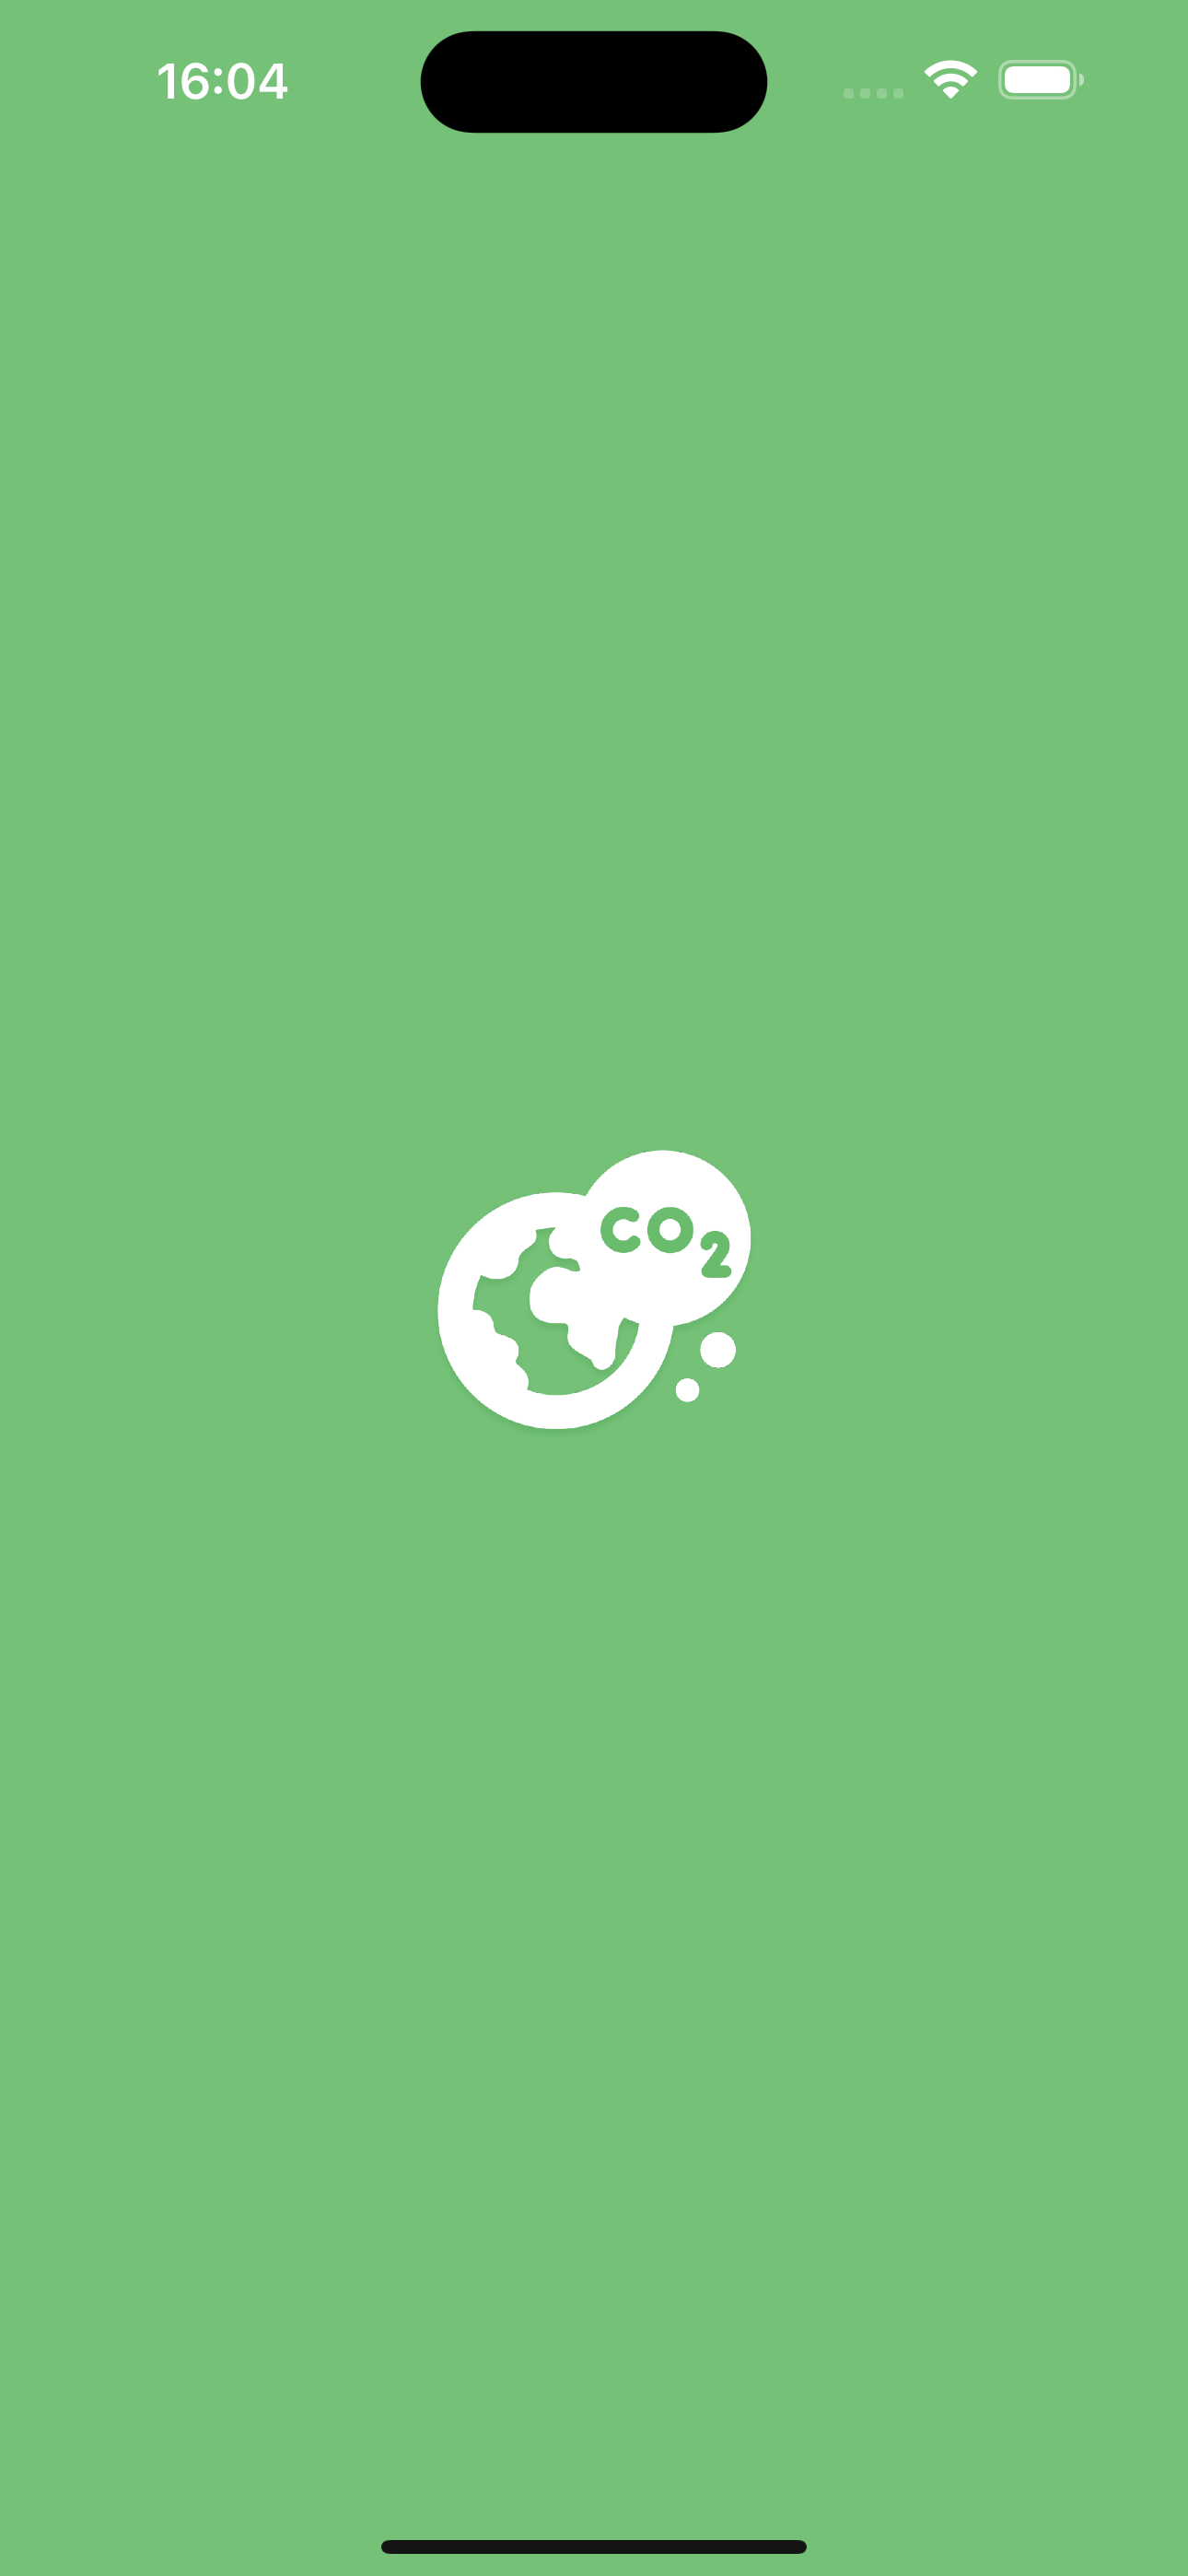
\includegraphics[width=0.45\textwidth]{Images/mobile/splash_screen.png}
  \caption[Màn hình chờ vào app]{\bfseries \fontsize{12pt}{0pt}
  \selectfont Màn hình chờ vào app}
  \label{splash_screen_waznet} %đặt tên cho ảnh
\end{figure}
\subsection{Các chức năng chung}
Tất cả các đối tượng sẽ có thể thực hiện được các chức năng chung sau:
\subsubsection{Chức năng đăng ký}
Người dùng sẽ phải nhập các thông tin và nhấn nút đăng ký. \textbf{Riêng với Admin} để đăng ký được cần có \textbf{một mã code} do bên nhà phát triển app cung cấp.

Một số lưu ý khi đăng ký:

\begin{adjustwidth}{1.5em}{}
  \begin{itemize}
    \item Họ và tên: phải điền một trong hai, không được để trống
    \item Số điện thoại: phải điền đúng format \textbf{10 số} (không kèm mã vùng)
    \item Mật khẩu: \textbf{đủ 8} ký tự trở lên
  \end{itemize}
\end{adjustwidth}
% \begin{figure}[H]
%   \centering
%   \includegraphics[width=12cm,height=3cm]{Images/mobile/}
%   \caption[Logo Firebase]{\bfseries \fontsize{12pt}{0pt}
%   \selectfont Logo Firebase}
%   \label{firebase_cover} %đặt tên cho ảnh
% \end{figure}
\begin{figure}[H]
  \centering
  \subcaptionbox{Màn đăng ký}{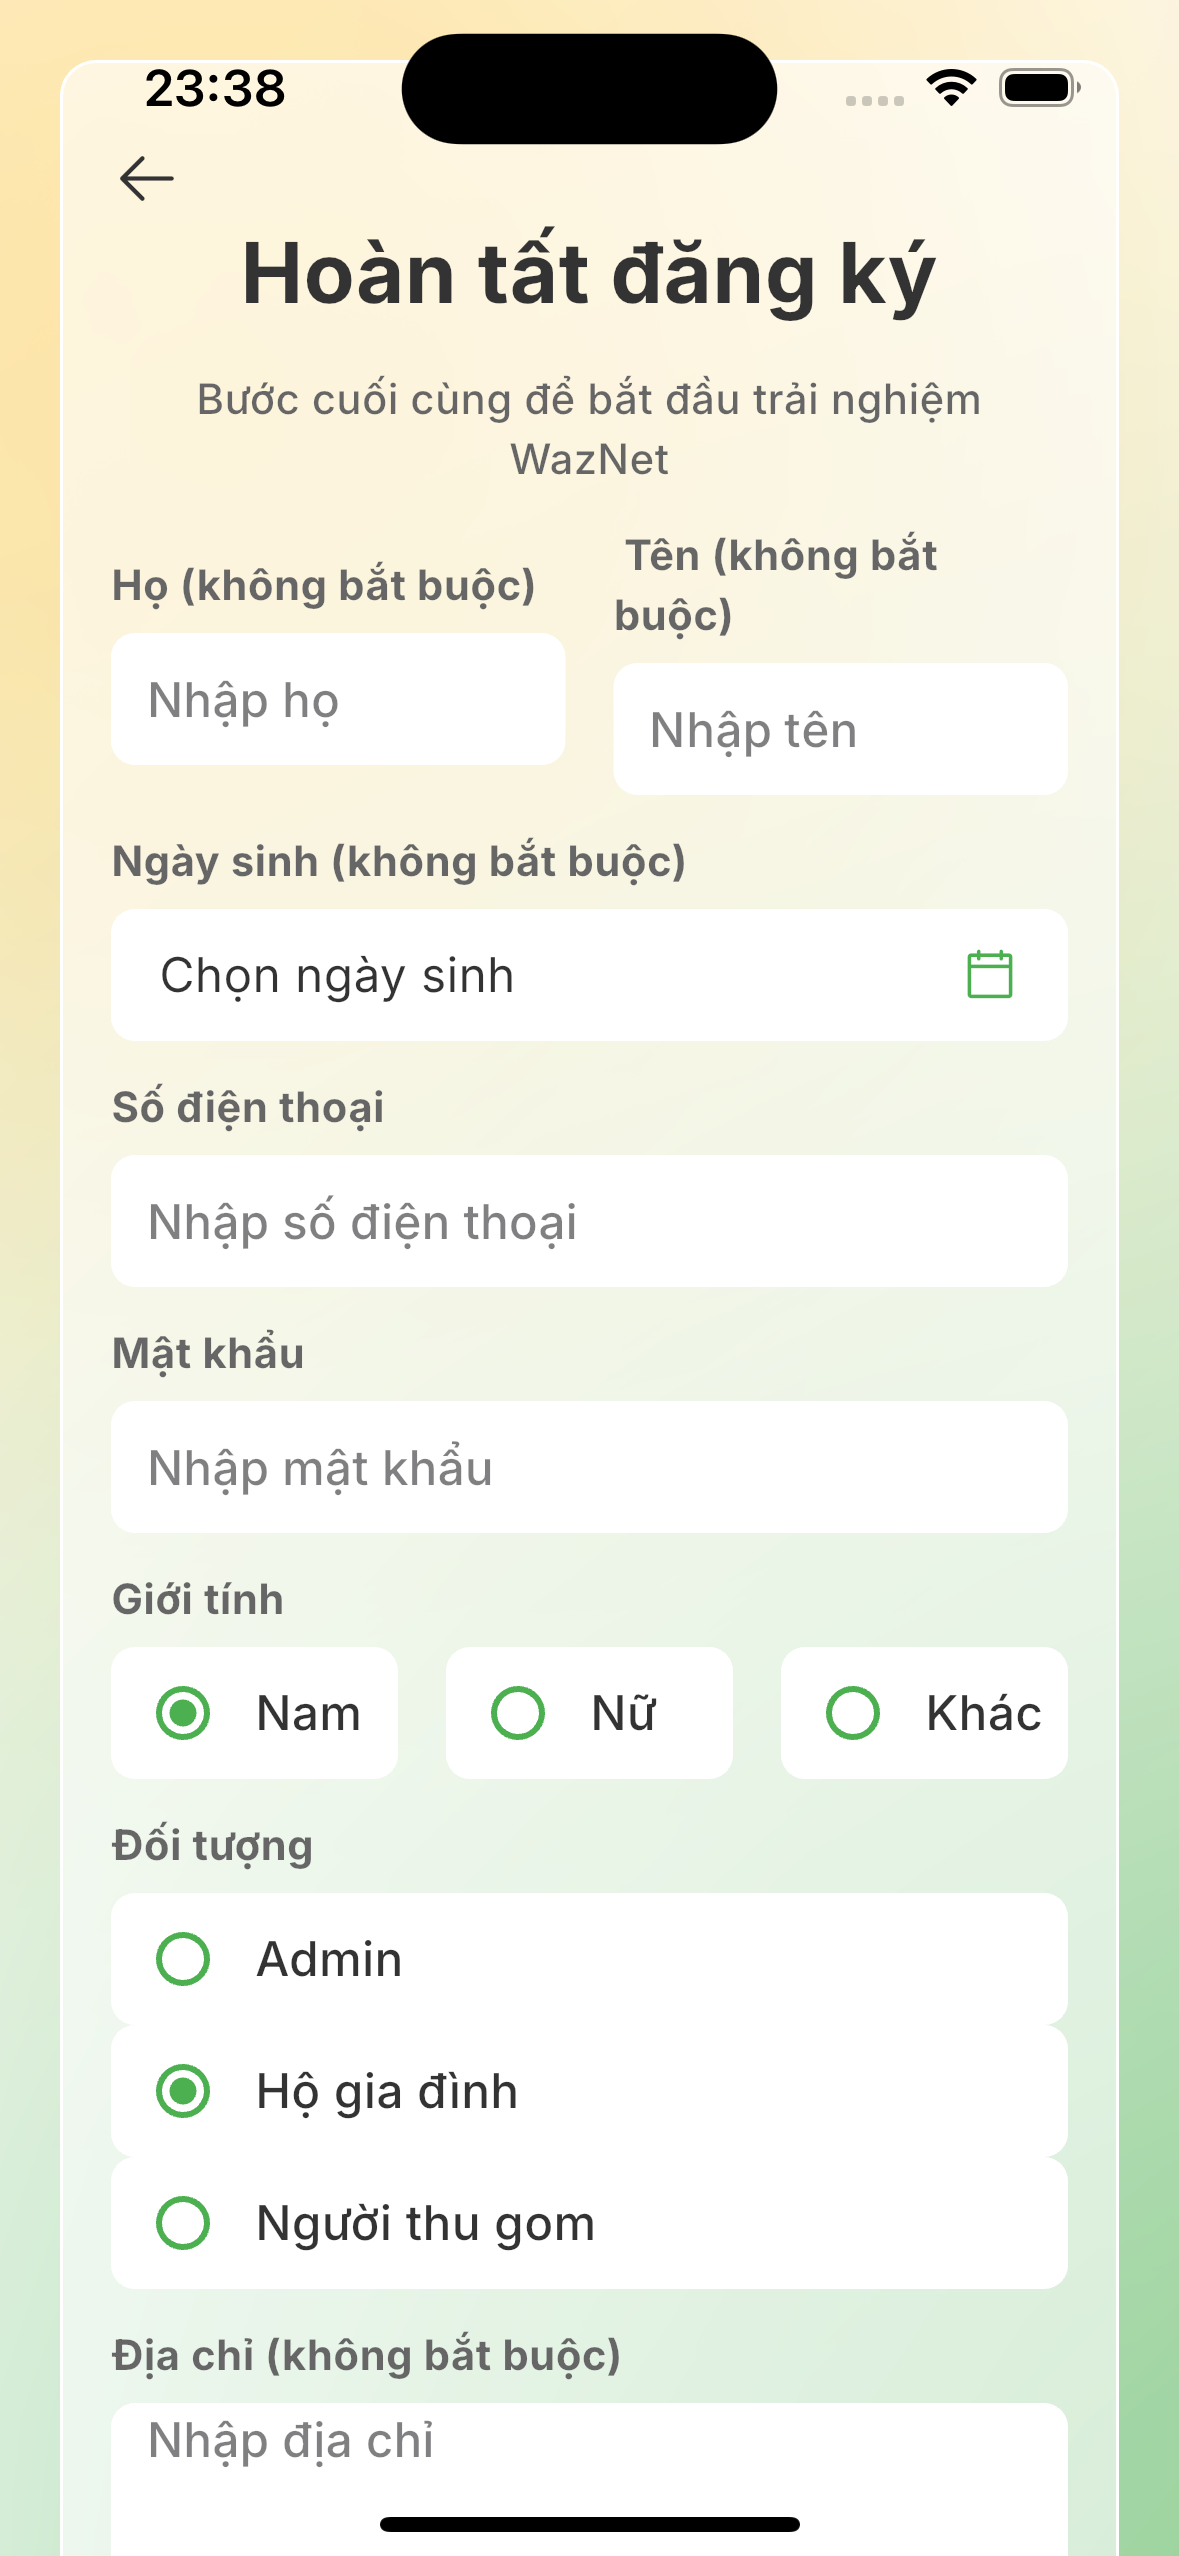
\includegraphics[width=0.45\textwidth]{Images/mobile/register_screen.png}}%
  \hfill
  \subcaptionbox{Màn đăng ký (tiếp)}{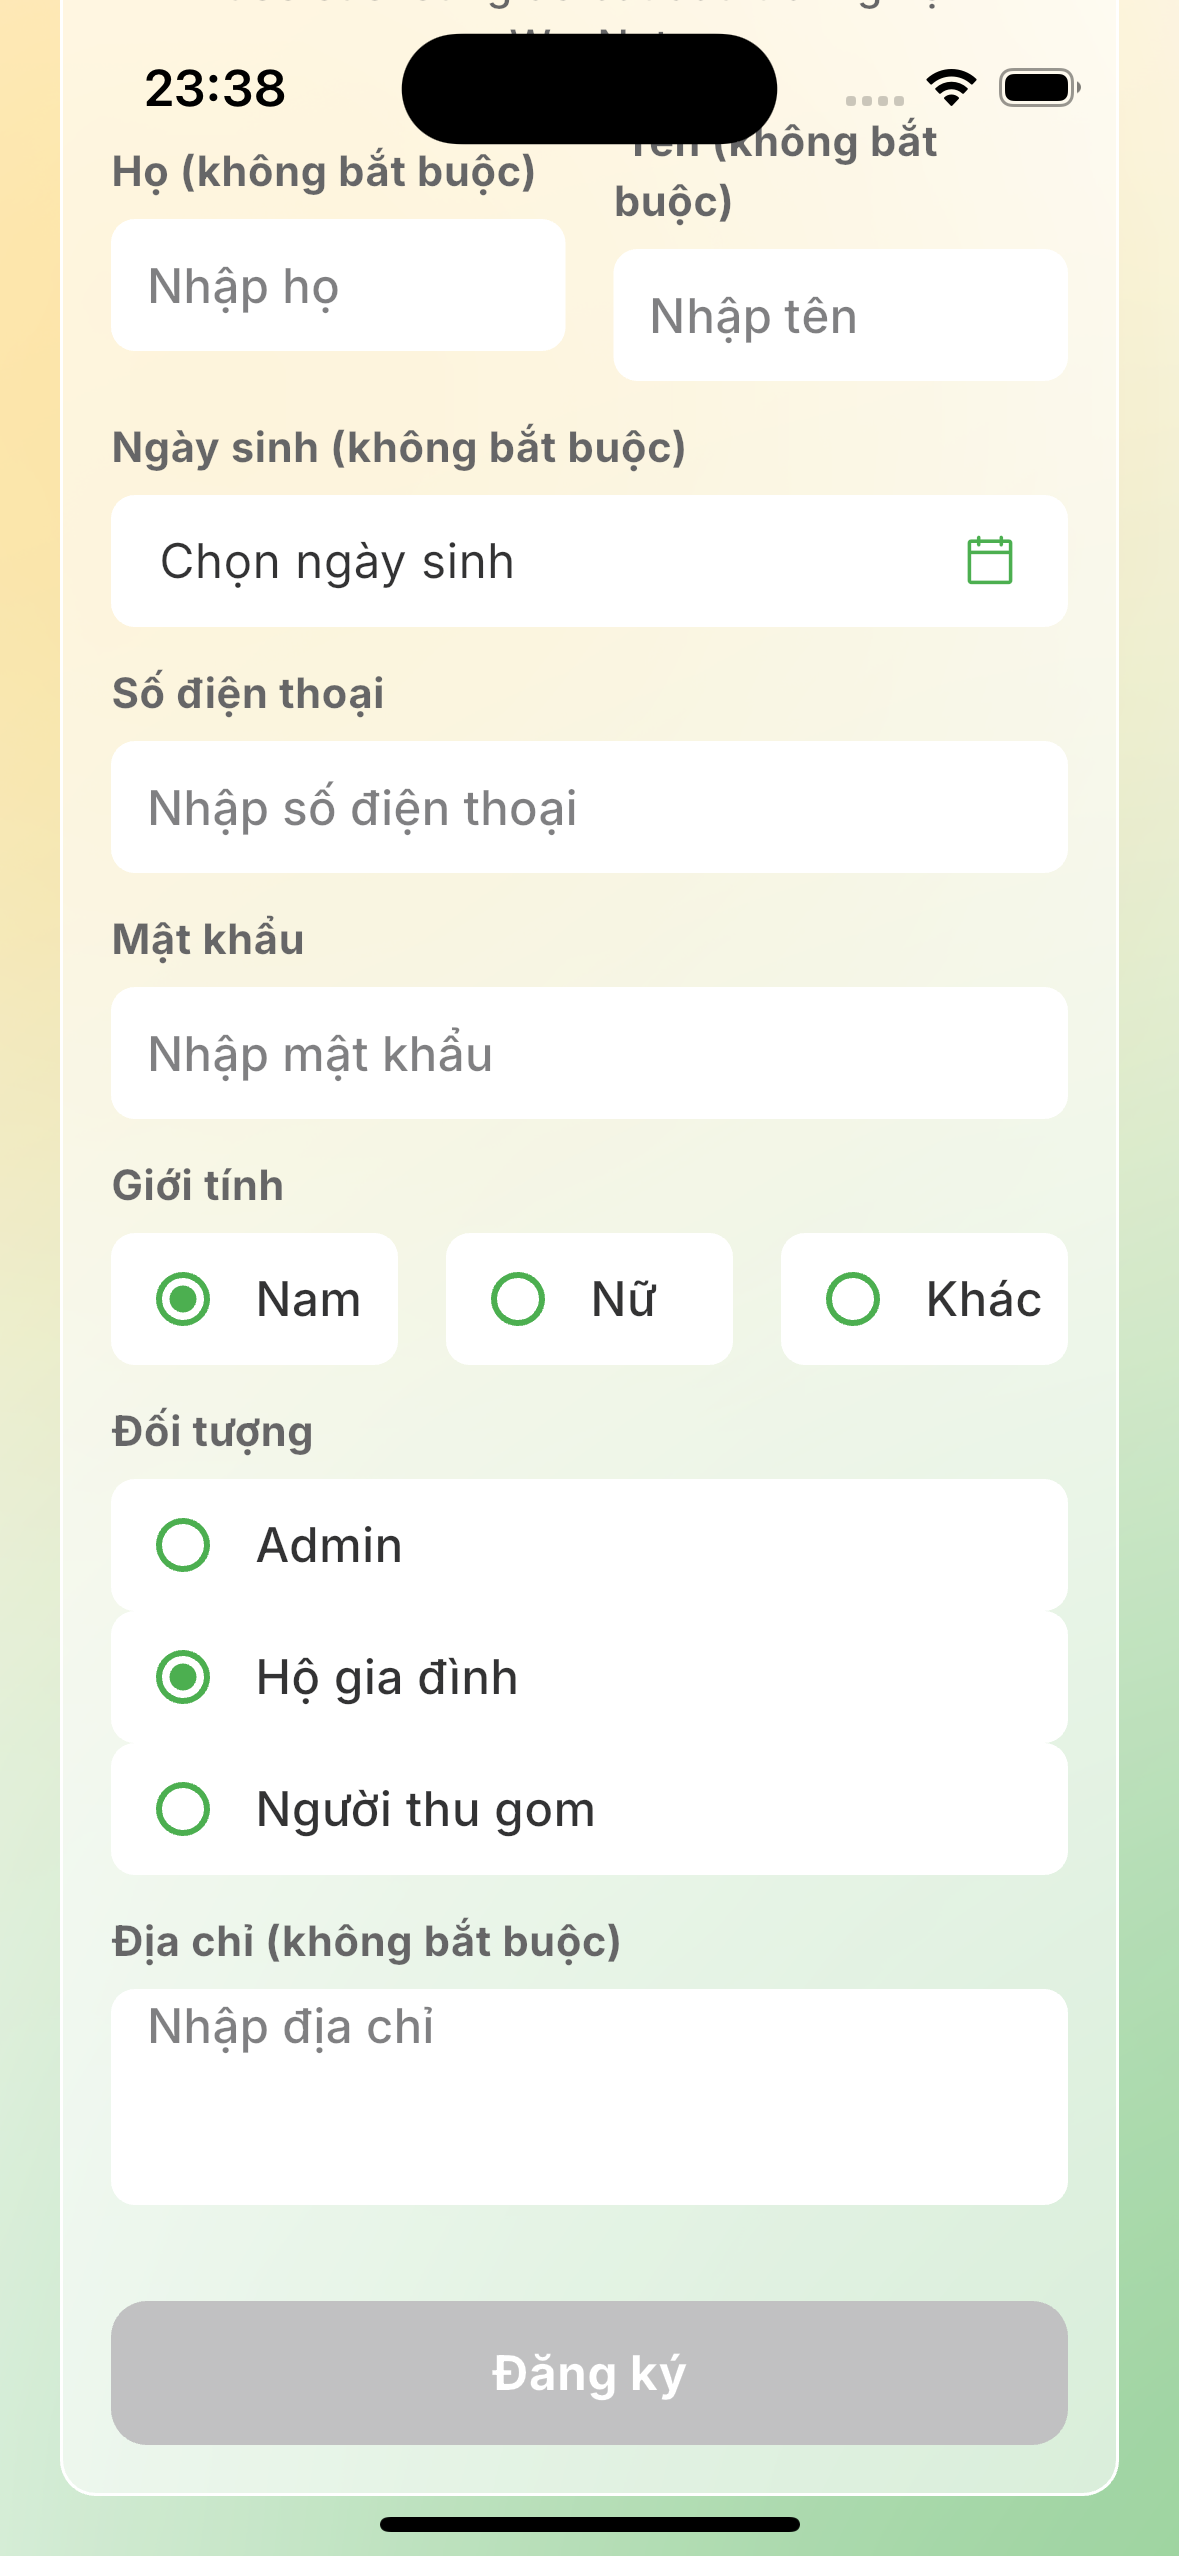
\includegraphics[width=0.45\textwidth]{Images/mobile/register_screen_2.png}}%
  \caption[Hình ảnh màn đăng ký]{\bfseries \fontsize{12pt}{0pt}
  \selectfont Hình ảnh màn đăng ký}
  \label{register_screen_waznet}
\end{figure}

% \begin{figure*}[ht!]
%   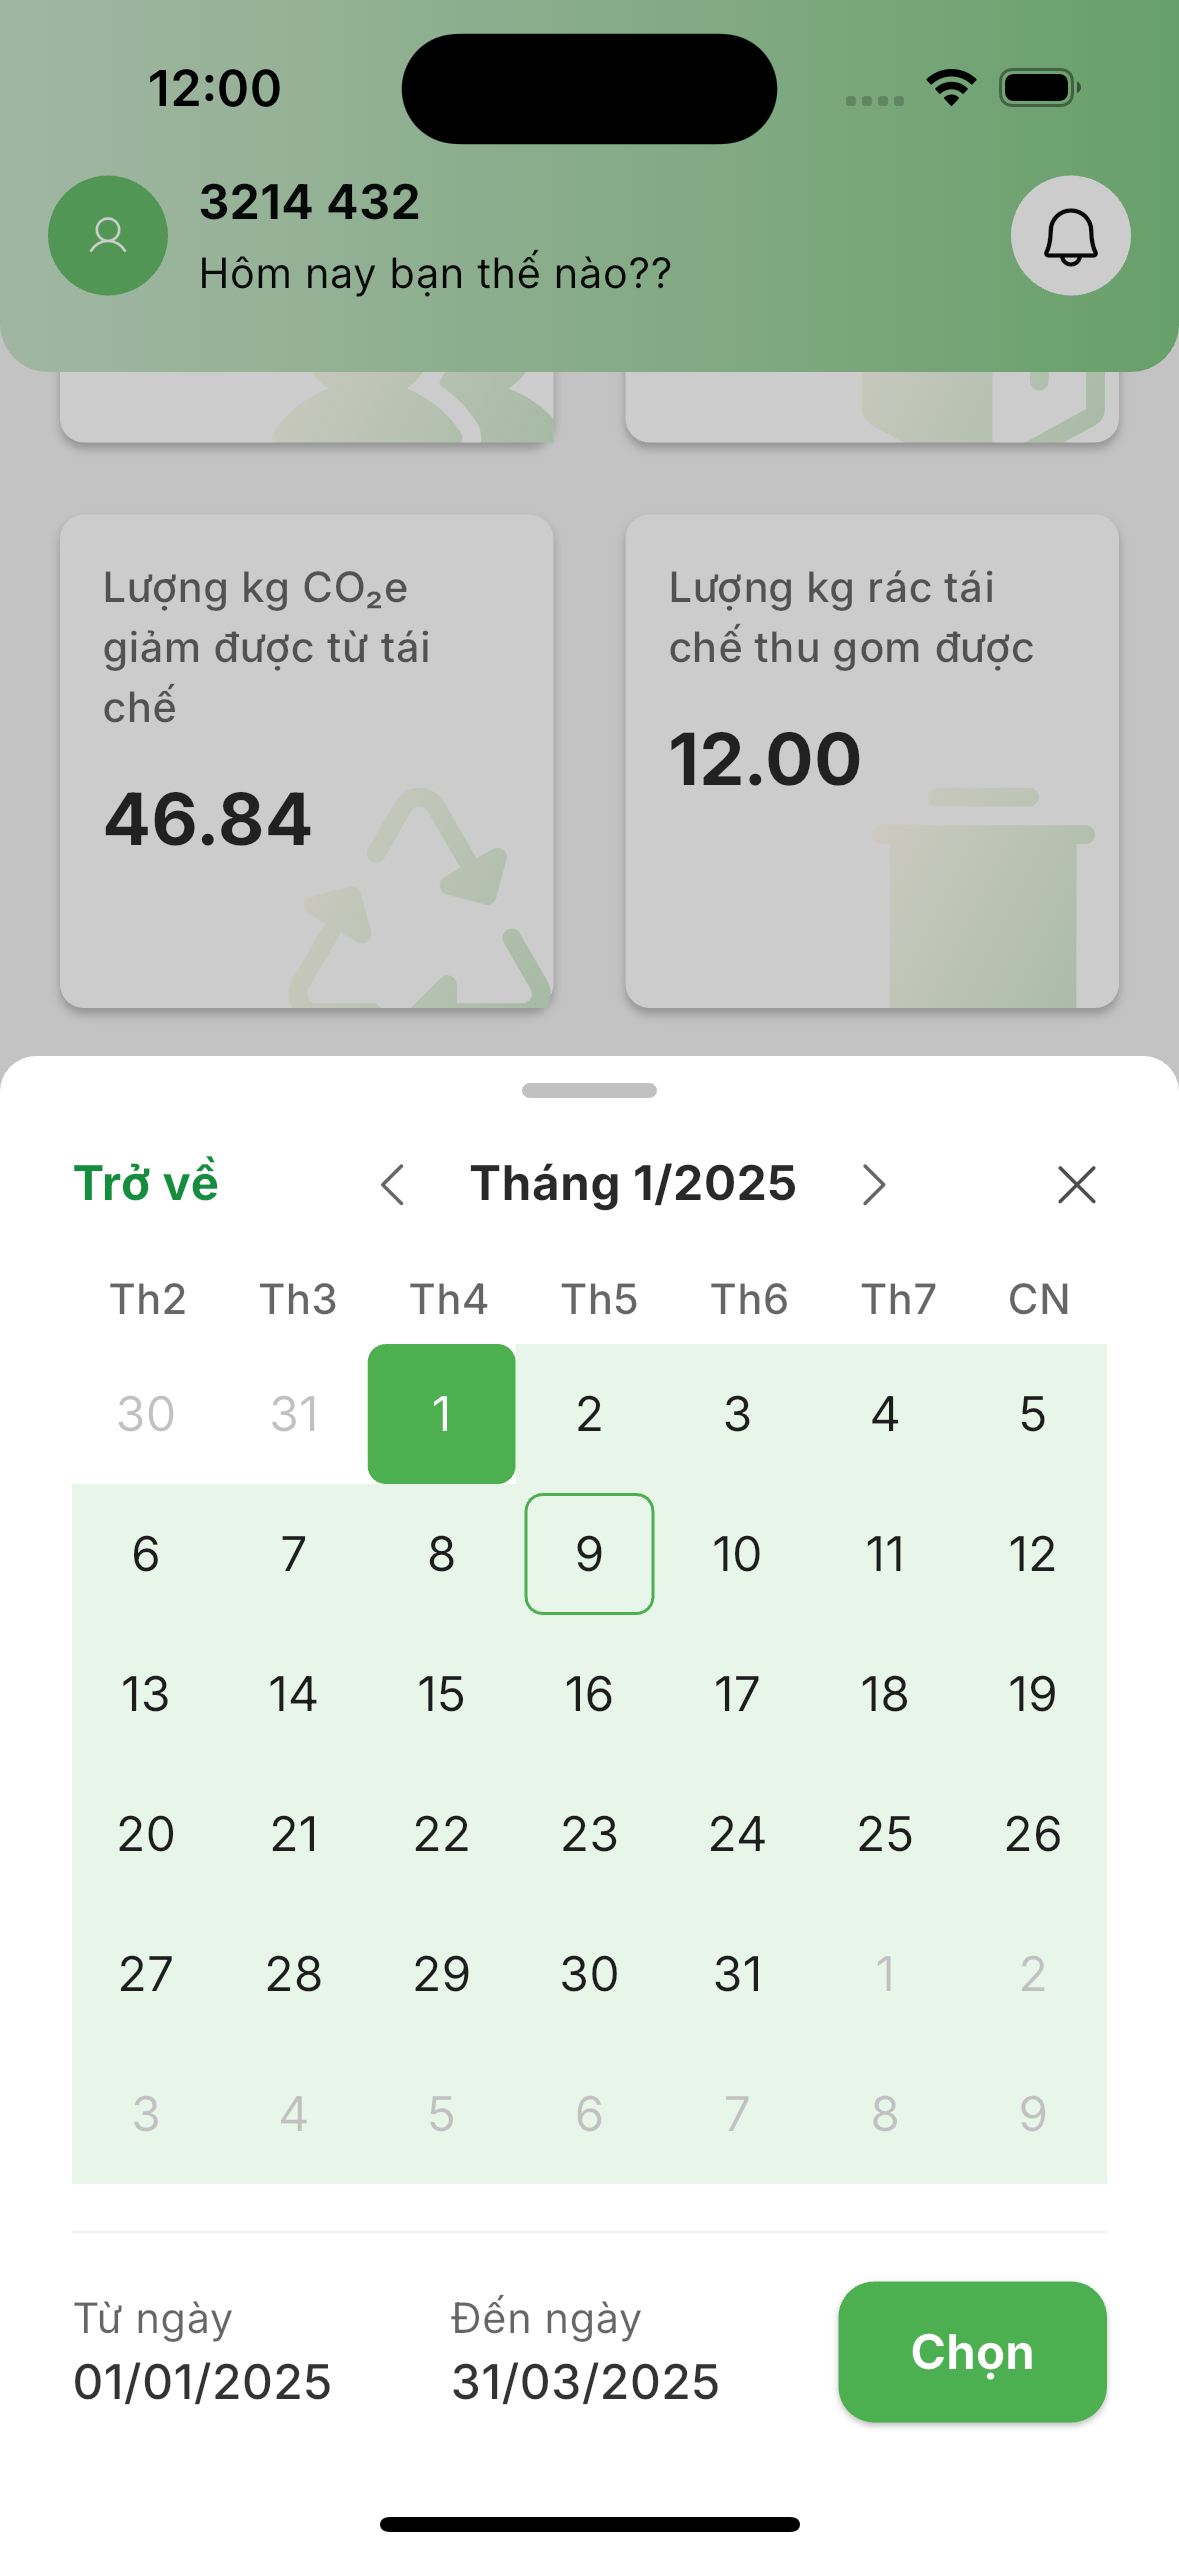
\includegraphics[width=.3\textwidth]{Images/mobile/filter_date.png}\hfill
%   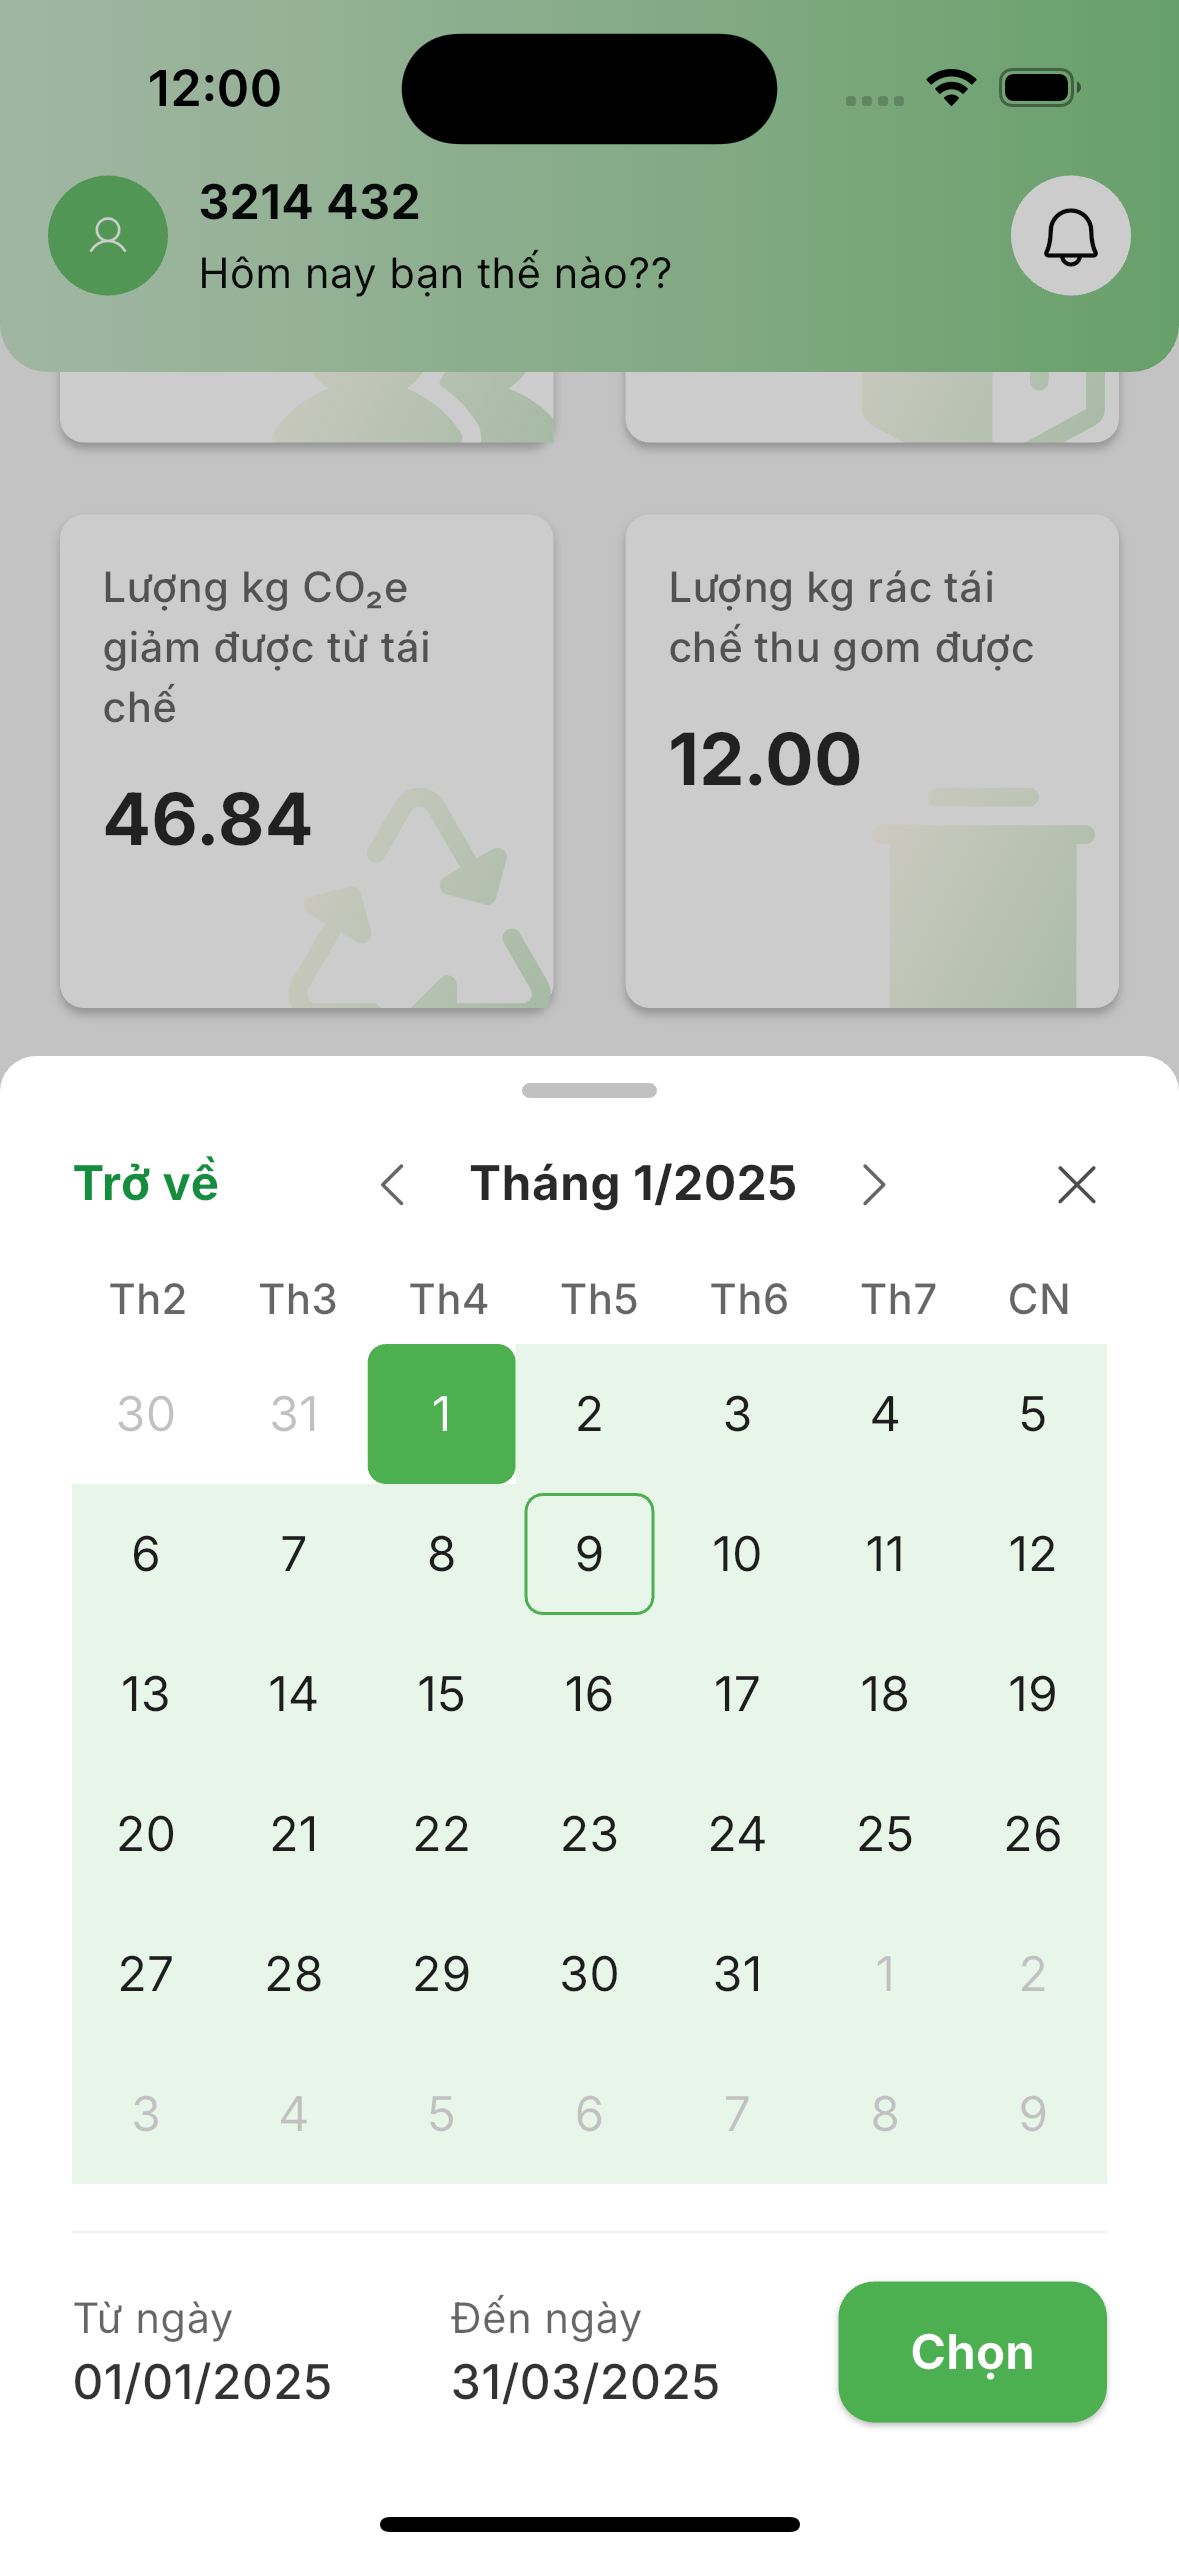
\includegraphics[width=.3\textwidth]{Images/mobile/filter_date.png}\hfill
%   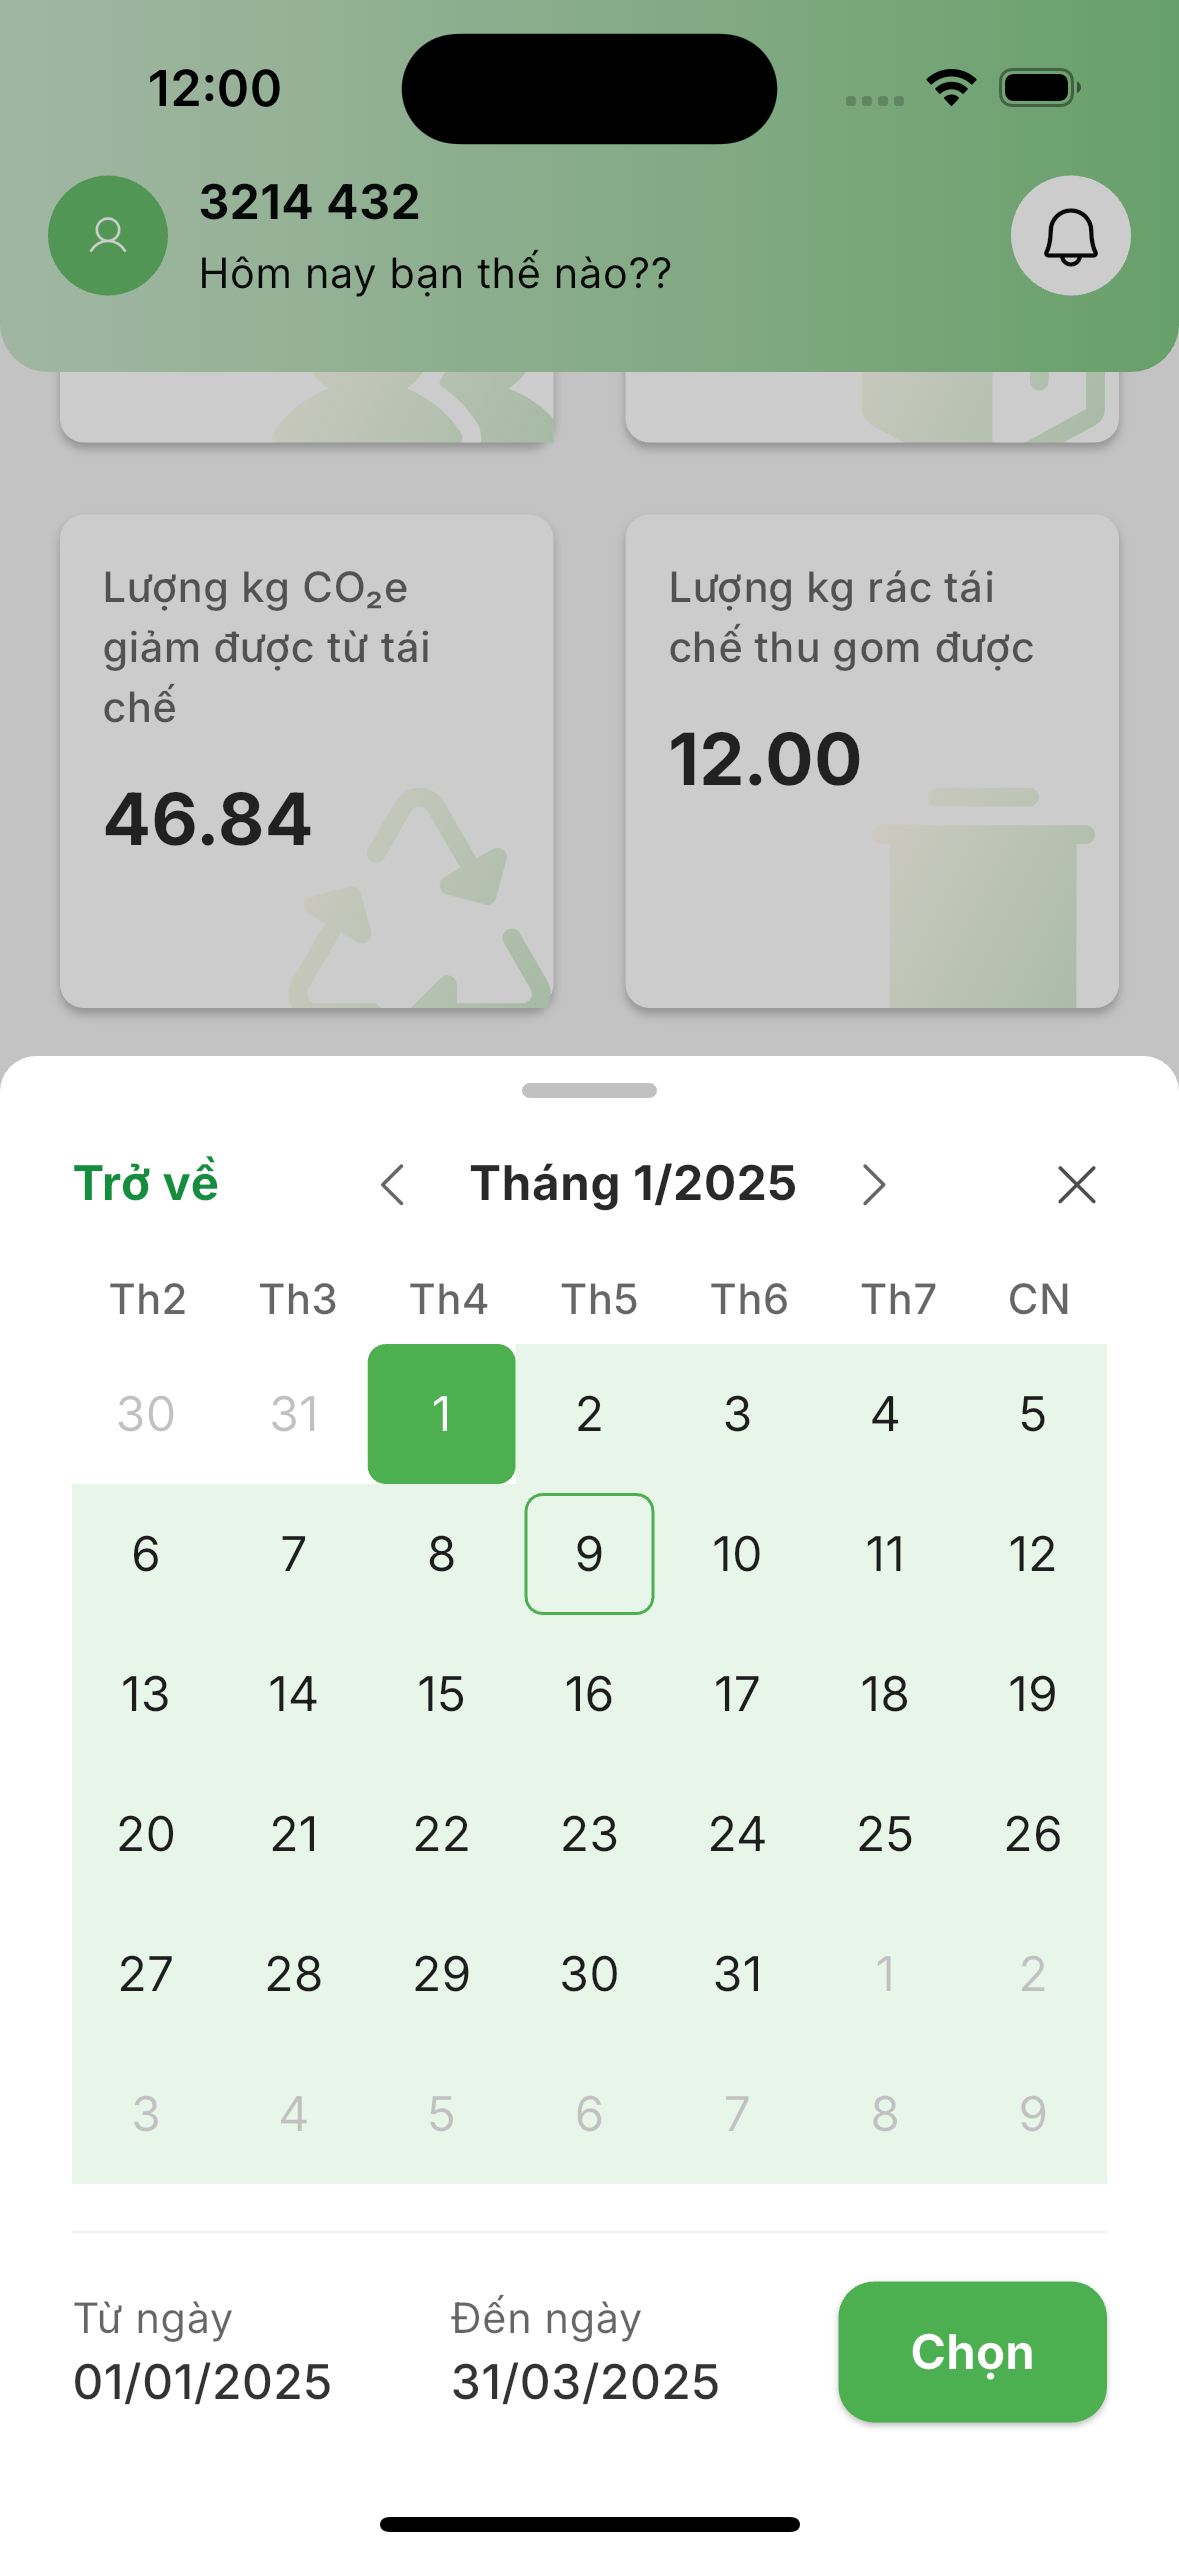
\includegraphics[width=.3\textwidth]{Images/mobile/filter_date.png}
%   \caption{Image A.}
%   \caption{Image B.}
%   \caption{Image C.}
% \end{figure*}

\subsubsection{Chức năng đăng nhập}
Người dùng sẽ phải nhập số điện thoại và mật khẩu để đăng nhập.
\begin{figure}[H]
  \centering
  \subcaptionbox{Màn nhập số điện thoại}{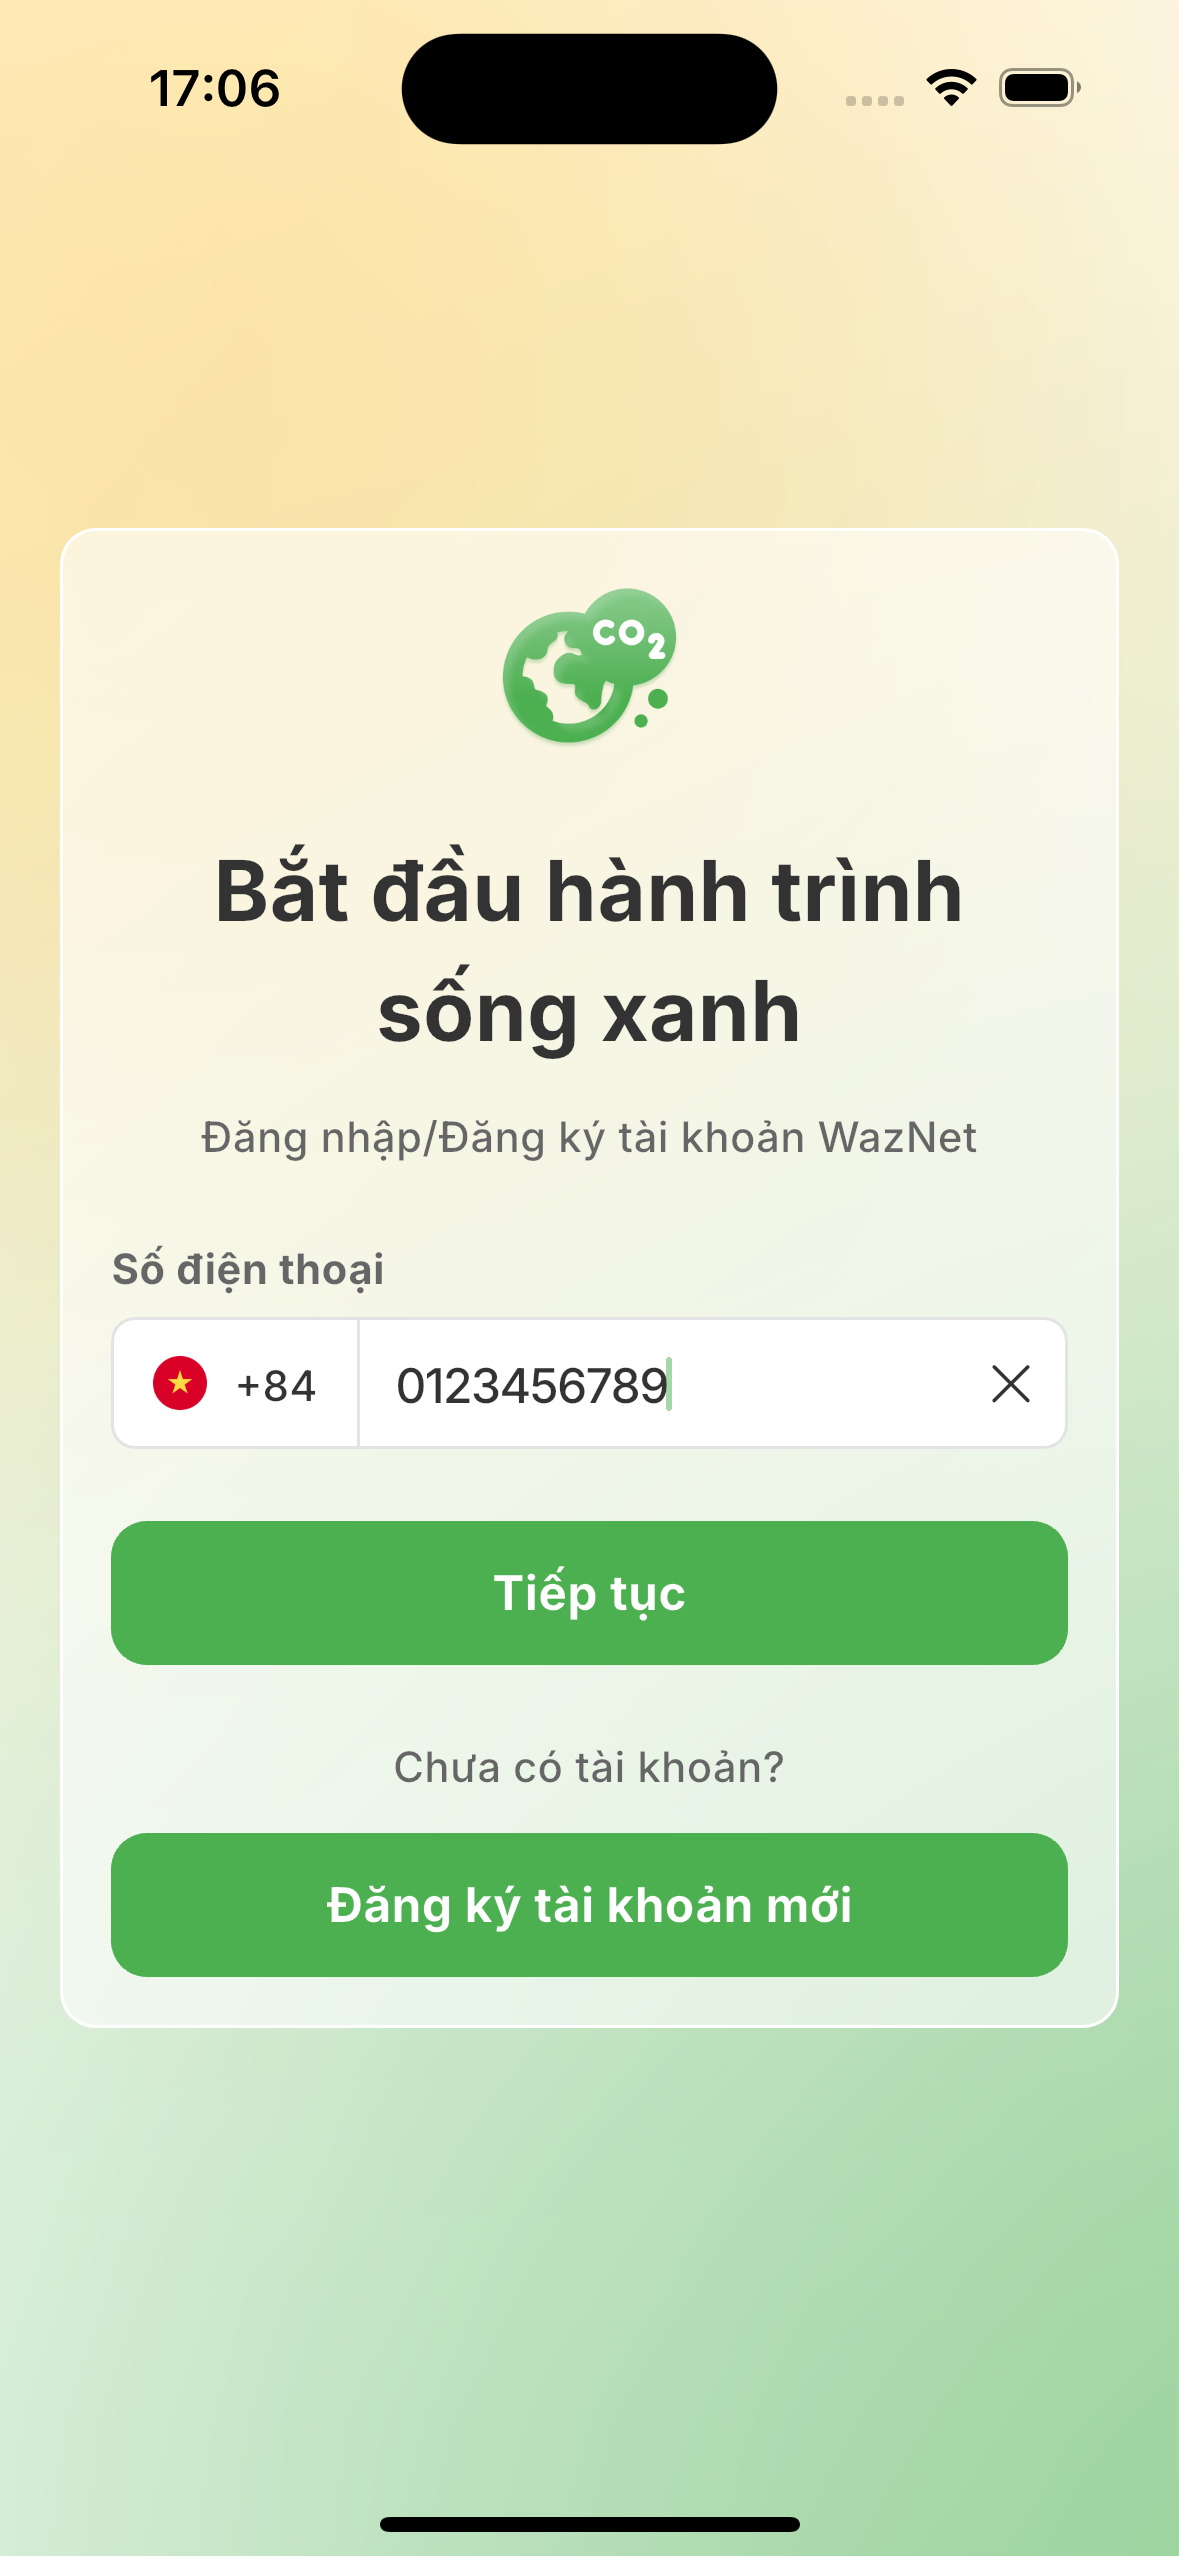
\includegraphics[width=0.32\textwidth]{Images/mobile/login_screen_1.png}}%
  \hfill
  \subcaptionbox{Màn nhập mật khẩu (lỗi)}{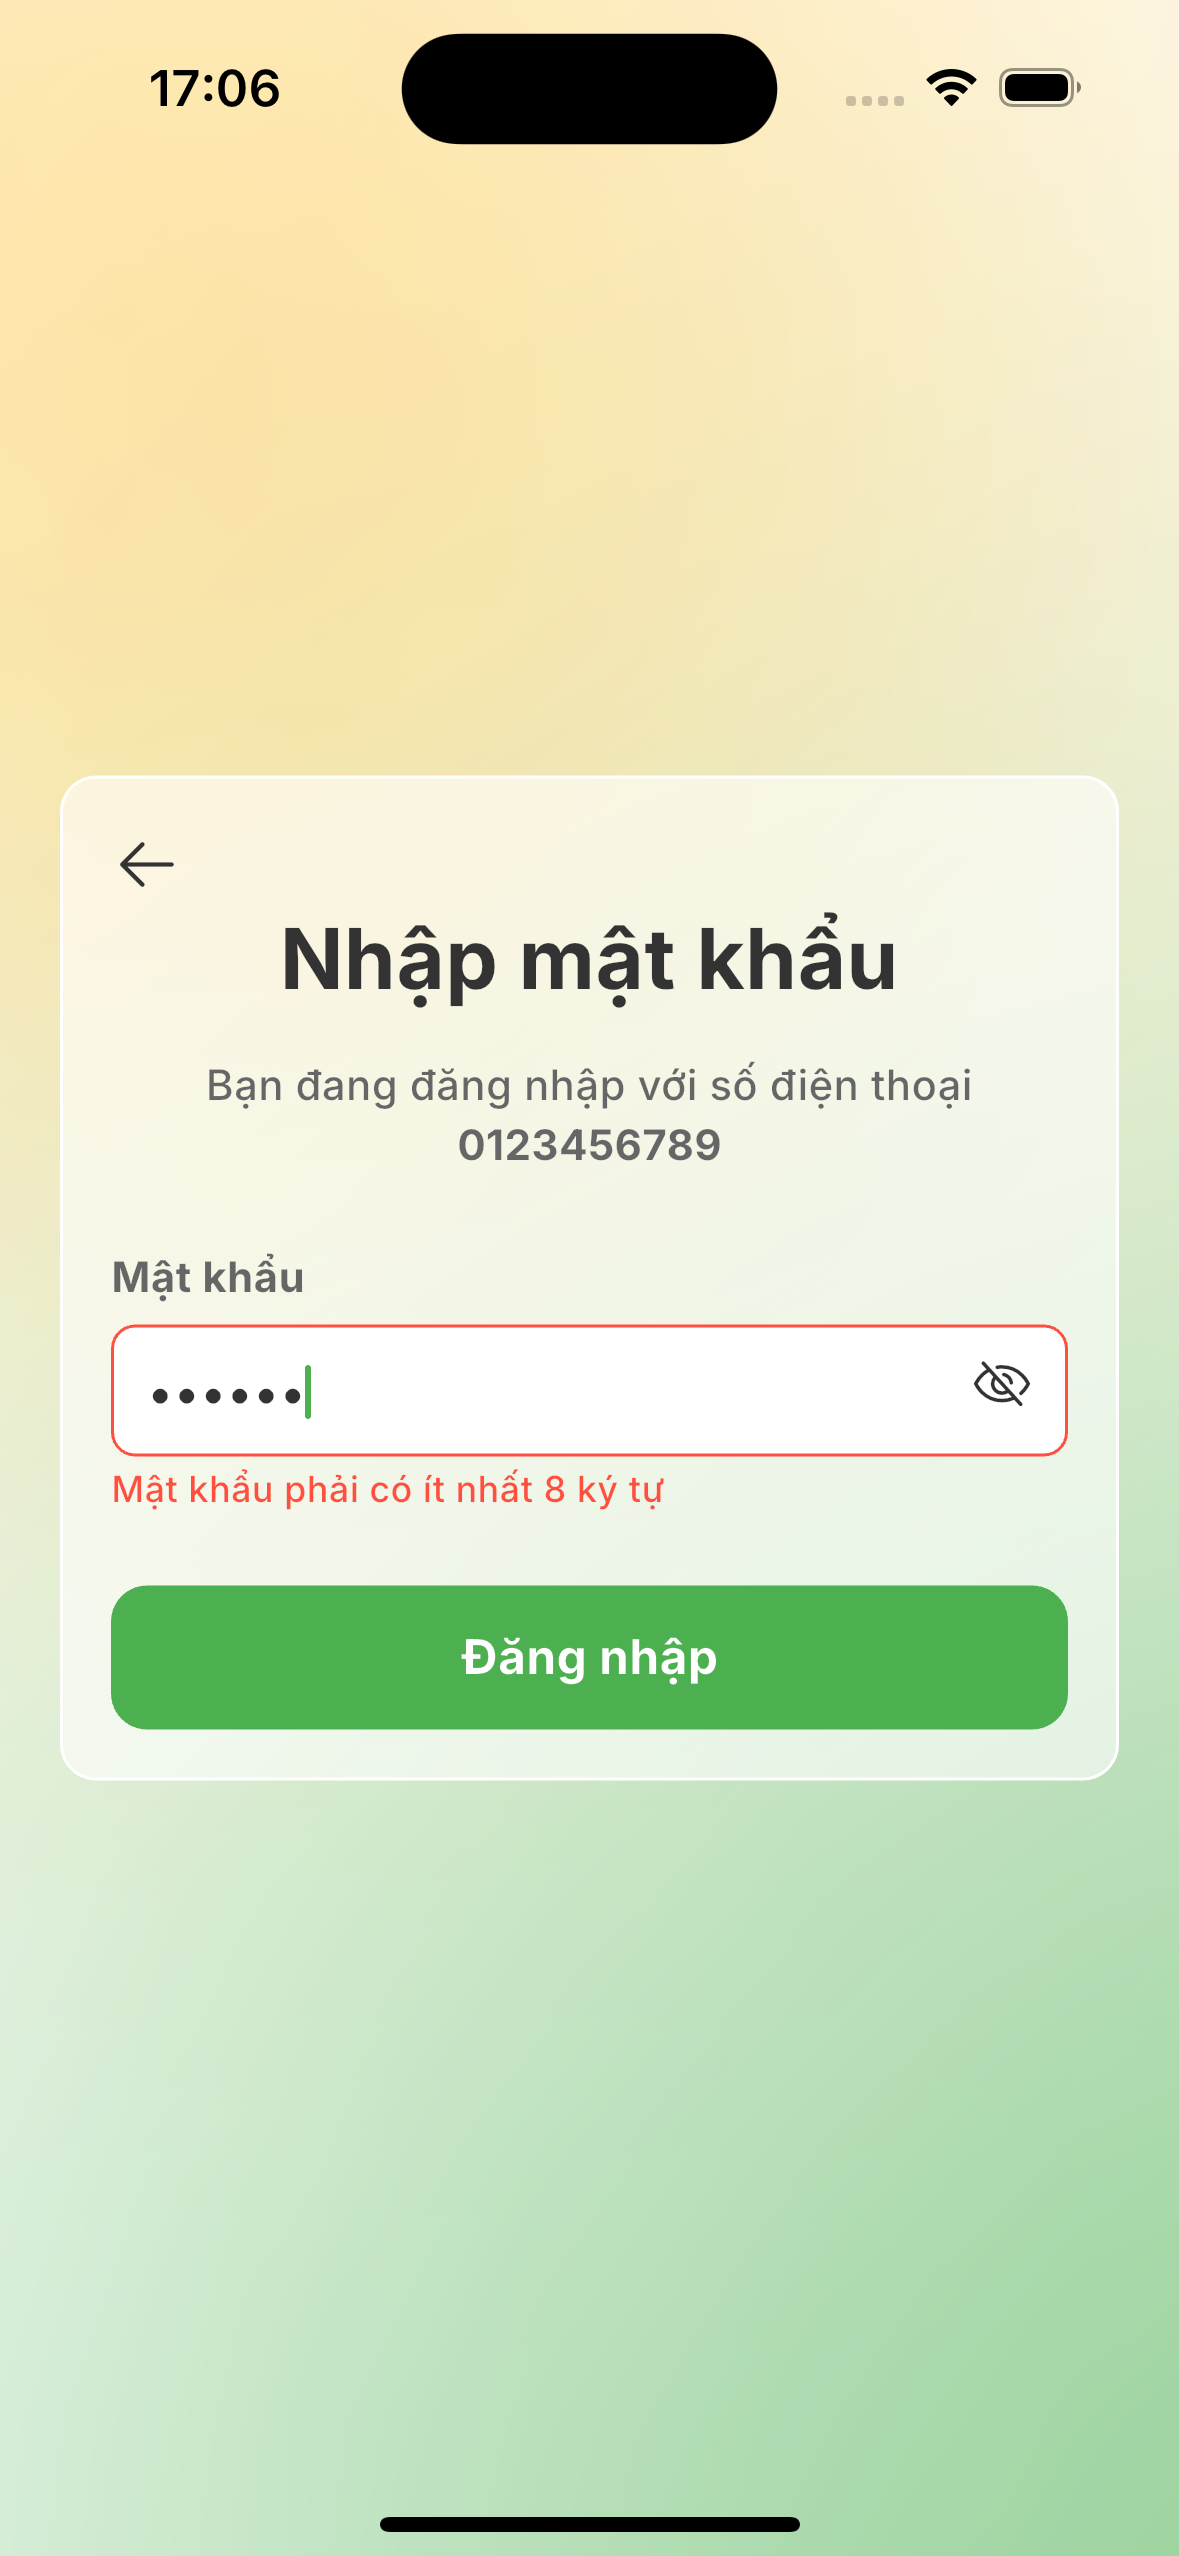
\includegraphics[width=0.32\textwidth]{Images/mobile/login_screen_2.png}}%
  \hfill
  \subcaptionbox{Màn đăng nhập (đủ ký tự)}{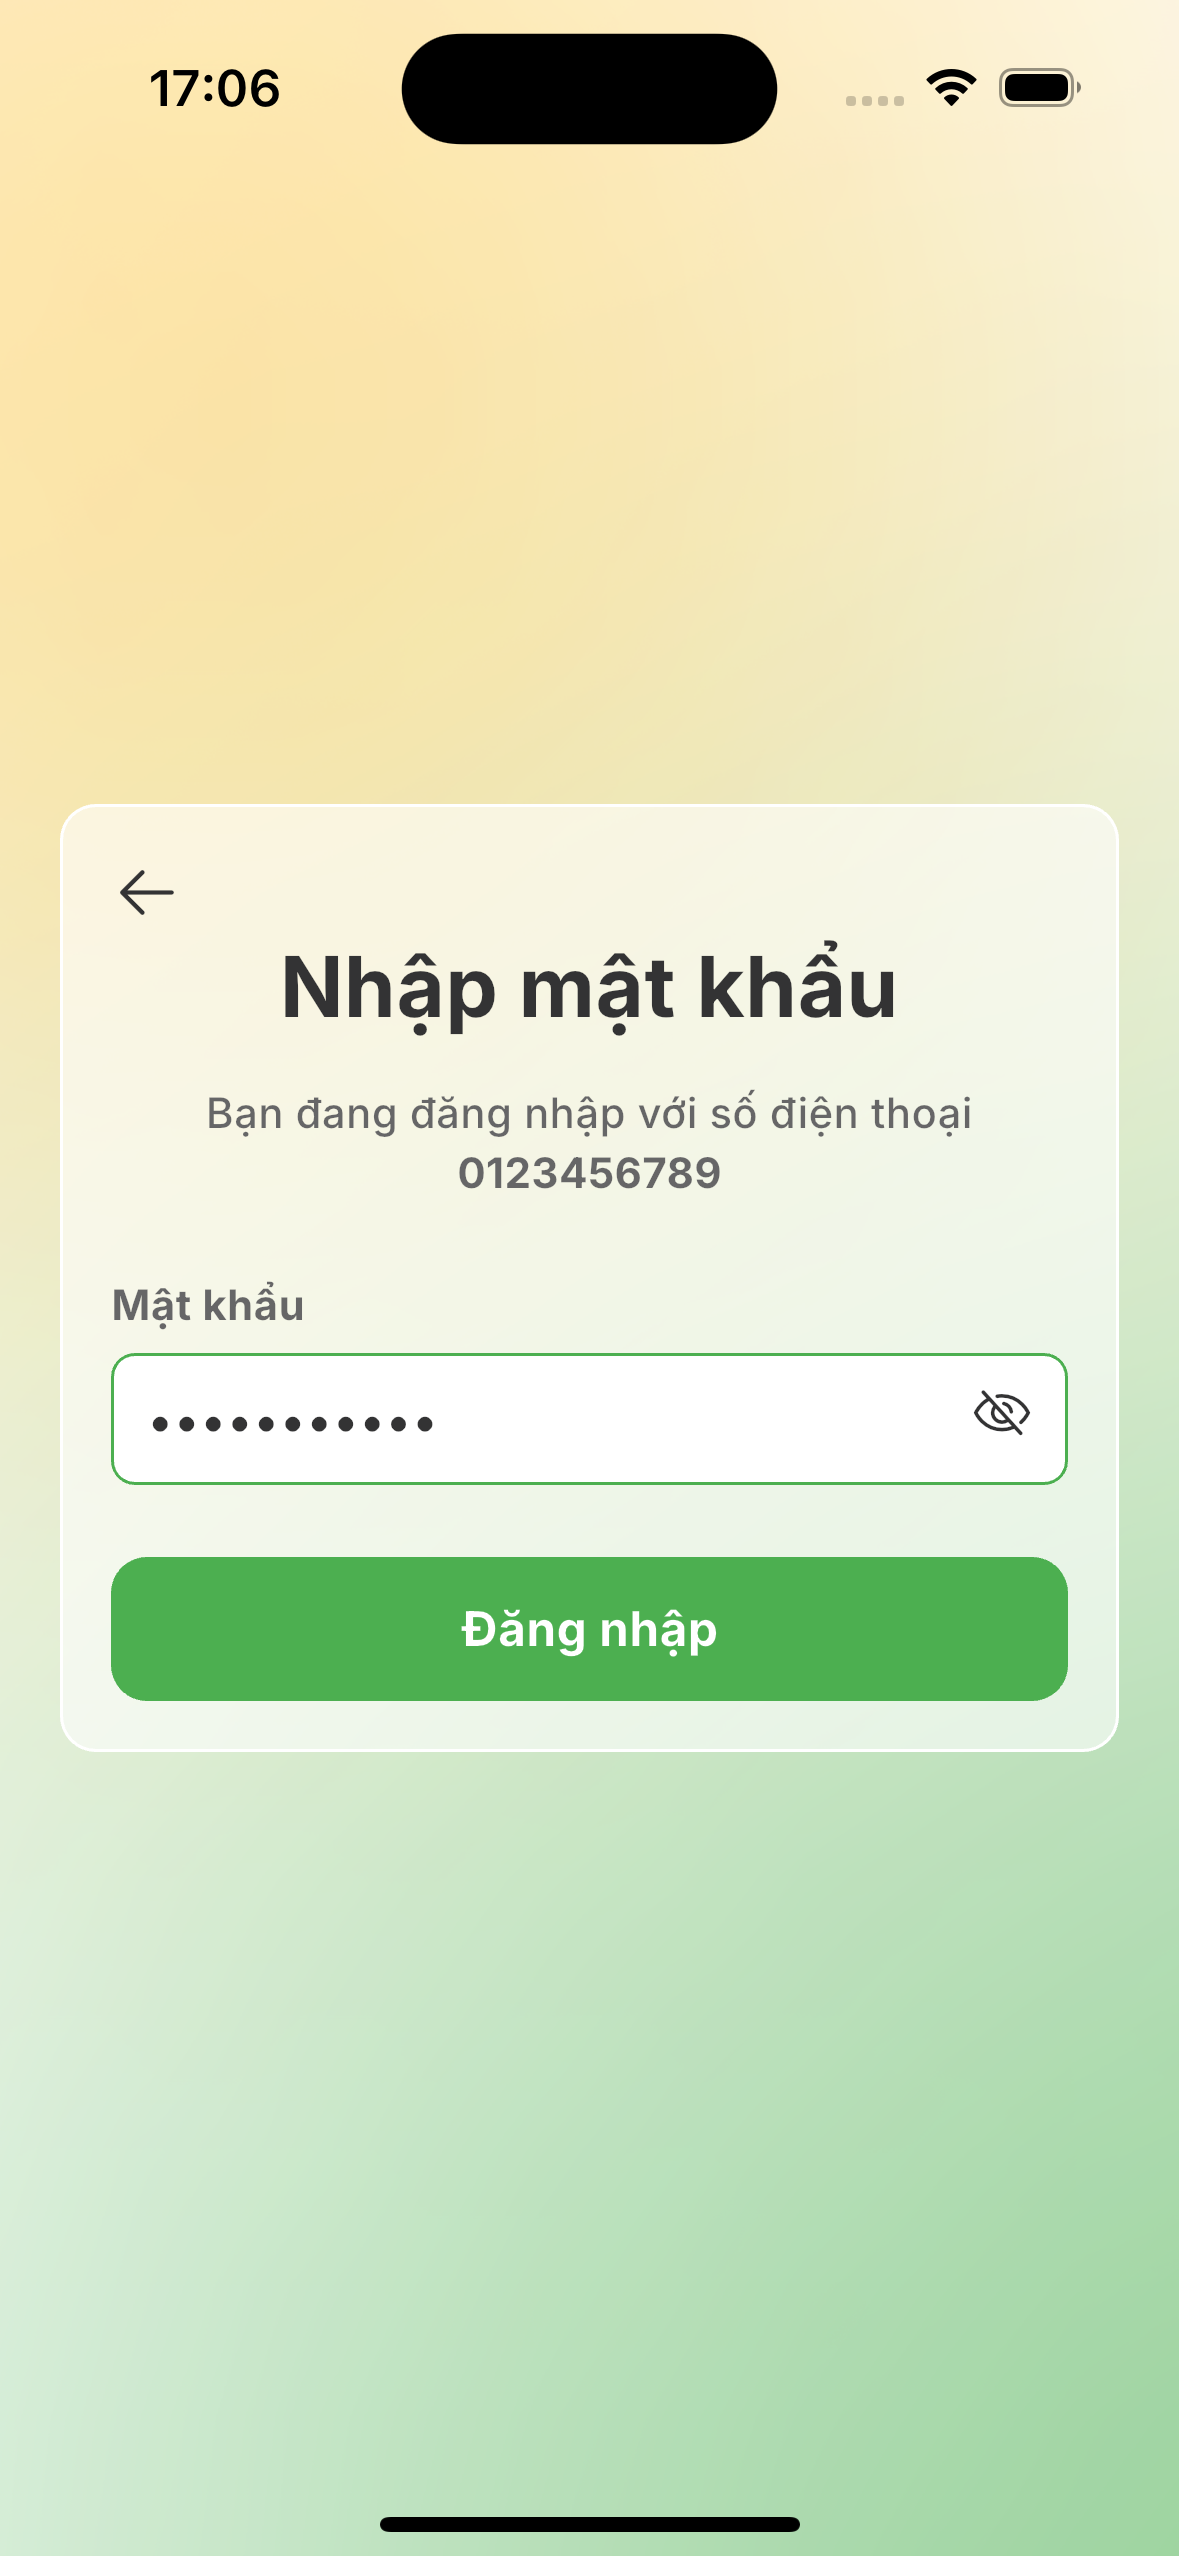
\includegraphics[width=0.32\textwidth]{Images/mobile/login_screen_3.png}}%
  \caption[Hình ảnh màn đăng nhập]{\bfseries \fontsize{12pt}{0pt}
  \selectfont Hình ảnh màn đăng nhập}
  \label{login_screen_waznet}
\end{figure}

\subsubsection{Chức năng xem chi tiết đóng góp đã nhập theo ngày}
Đối với Hộ gia đình và người thu gom, nhấn vào tab \textbf{Số liệu}, chọn một ngày, dữ liệu sẽ hiển thị như hình dưới
\begin{figure}[H]
  \centering
  \subcaptionbox{Màn danh sách đóng góp}{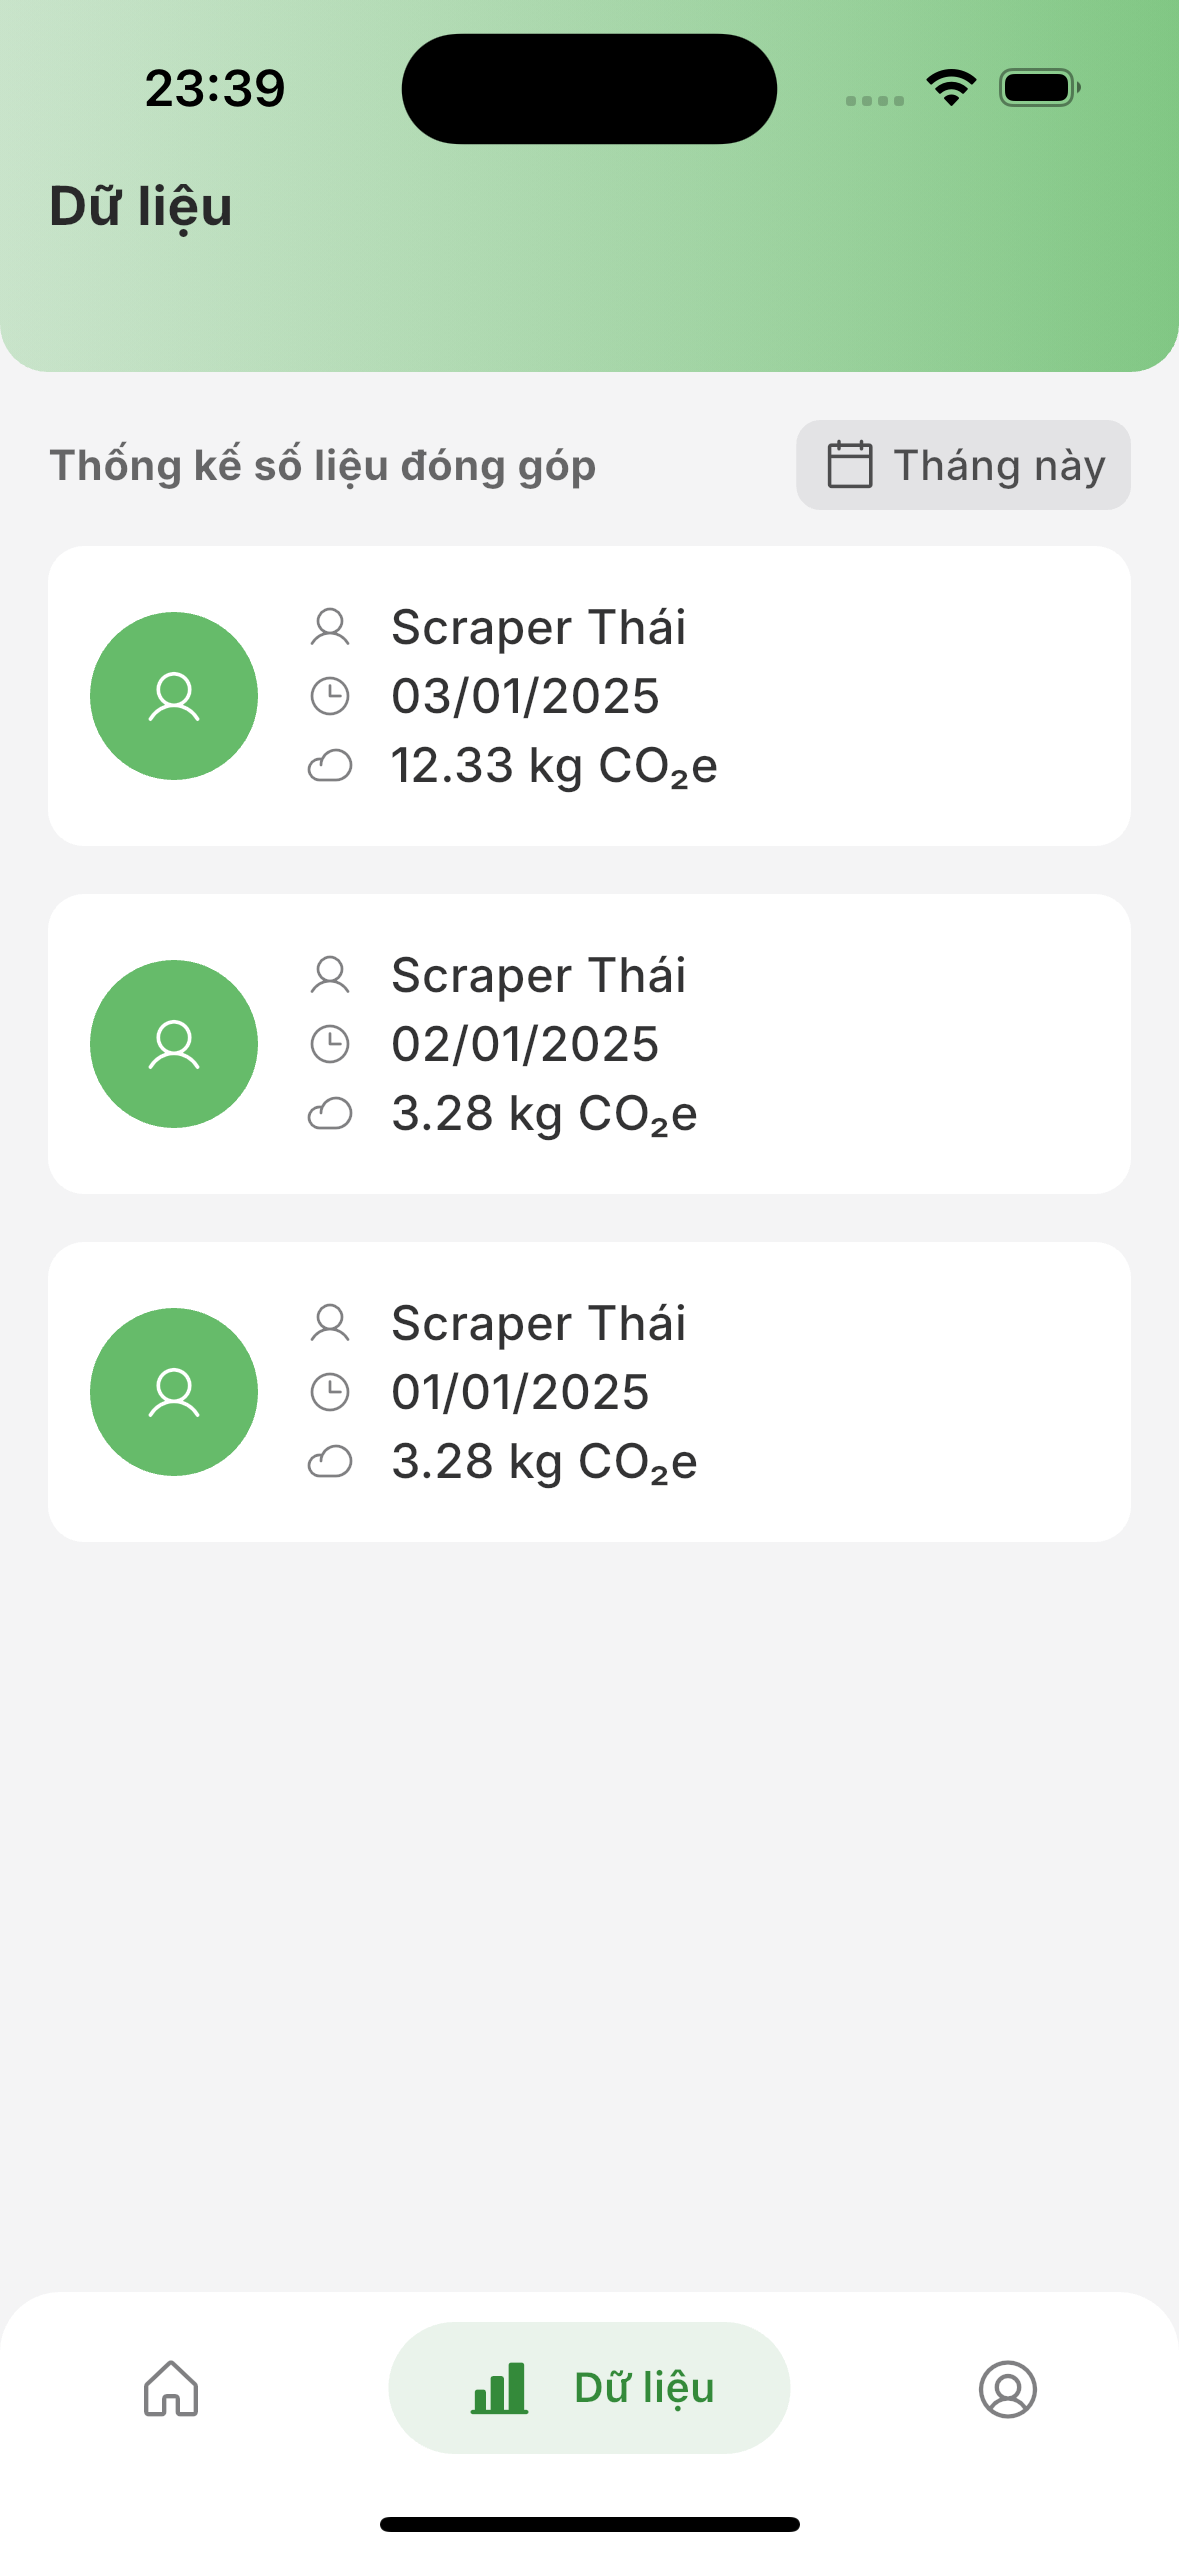
\includegraphics[width=0.45\textwidth]{Images/mobile/contributions_screen.png}}%
  \hfill
  \subcaptionbox{Màn chi tiết đóng góp trong một ngày}{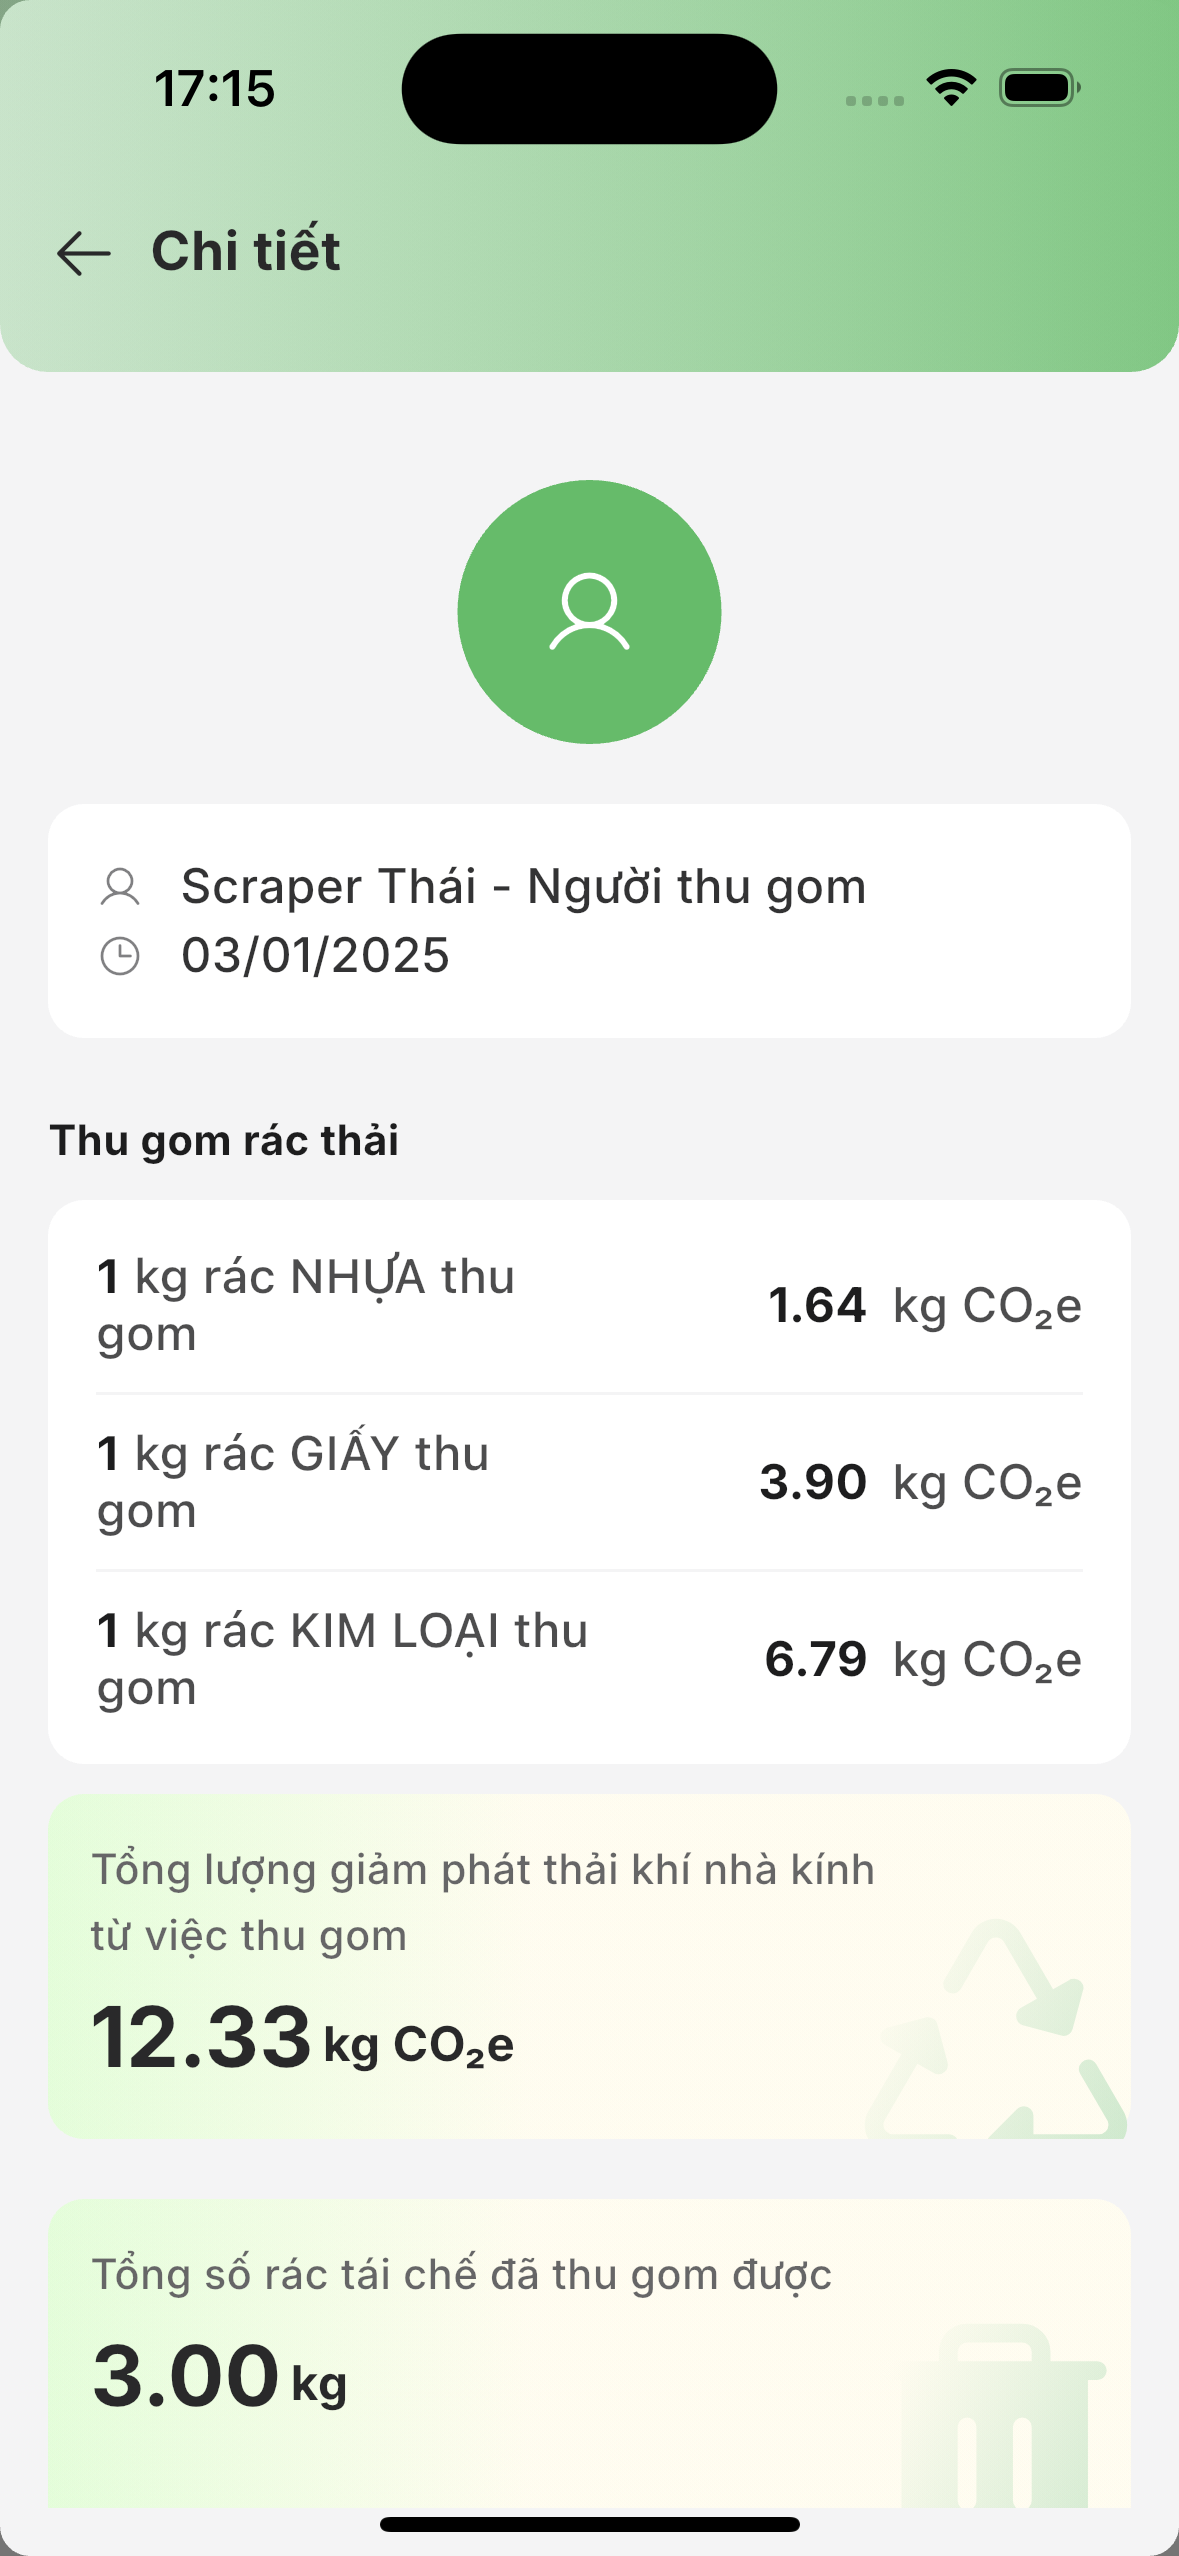
\includegraphics[width=0.45\textwidth]{Images/mobile/contribution_detail_screen.png}}%
  \caption[Hình ảnh màn thống kê/chi tiết đóng góp]{\bfseries \fontsize{12pt}{0pt}
  \selectfont Hình ảnh màn thống kê/chi tiết đóng góp}
  \label{contribution_screen_waznet}
\end{figure}

\subsubsection{Chức năng lọc số liệu đã nhập theo khoảng thời gian}
Đối với Hộ gia đình, nhấn vào tab \textbf{Số liệu}, bên cạnh dòng \textbf{Thống kê số liệu đóng góp}, 
\subsubsection{Chức năng sửa thông tin người dùng}
\subsubsection{Chức năng đổi ảnh đại diện}
\subsubsection{Chức năng đổi mật khẩu}
\subsubsection{Chức năng đăng xuất}
\subsubsection{Chức năng xoá tài khoản}

\subsection{Các chức năng riêng cho Hộ gia đình/Người thu gom}
\subsubsection{Chức năng nhập số liệu}
\subsubsection{Chức năng đăng ký nhận thông báo nhập liệu hàng ngày}

\subsection{Các chức năng riêng cho Admin}
\subsubsection{Chức năng xuất excel theo khoảng thời gian}

\newpage